%%%%%%%%%%%%%%%%%%%%%%%%%%%%%%%%%%%%%%%%%%%%%%%%%%%%%%%%%%%%%%%%%
%%% COSYNE-2007 摘要模板
%%% 版本 1.0
%%%%%%%%%%%%%%%%%%%%%%%%%%%%%%%%%

\documentclass[12pt]{article}
\usepackage{listings}
\usepackage{xeCJK}  % 支持中文
\usepackage{fontspec}
\usepackage{xcolor} % 定义颜色

% 定义背景颜色和代码相关颜色
\definecolor{backcolour}{rgb}{0.95,0.95,0.92} % 浅灰色背景
\definecolor{codegreen}{rgb}{0,0.6,0}
\definecolor{codegray}{rgb}{0.5,0.5,0.5}
\definecolor{codepurple}{rgb}{0.58,0,0.82}

\lstset{
    backgroundcolor=\color{backcolour},   
    commentstyle=\color{codegreen},
    keywordstyle=\color{blue},
    numberstyle=\tiny\color{codegray},
    stringstyle=\color{codepurple},
    basicstyle=\ttfamily\small,
    breakatwhitespace=false,         
    breaklines=true,                 
    keepspaces=true,                 
    numbers=left,                    
    numbersep=5pt,                  
    showspaces=false,                
    showstringspaces=false,
    showtabs=false,                  
    tabsize=2,
    frame=single,
    inputencoding=utf8,
    extendedchars=true,
    upquote=true,                    % 修正引号显示
    columns=flexible,                % 保持代码格式
    keepspaces=true,                 % 保持空格
    basewidth={0.5em,0.5em},         % 等宽字符
    escapechar=@,                    % 设置转义字符
    literate=                        % 正确显示下划线
        {_}{{\textunderscore}}1
        {-}{{-}}1
        {~}{{\textasciitilde}}1
}

\usepackage{amssymb} %数学符号
\usepackage{amsmath} %数学公式
\usepackage{graphicx}
\usepackage{hyperref}
\usepackage{color,soul}

\usepackage[margin=0.5in]{geometry}
\usepackage{times}
% 使中文能够正常显示
\usepackage{CJKutf8}

\parindent 0pt
\parskip 0pt

\pagestyle{empty}		% 无页码

\begin{document}




%%%----------------------------------------------------------------- 
{\bf \large
结合漏电积分放电模型与电缆方程的神经元仿真
}\\
{ 杨博 221900435 
}\\

%%%----------------------------------------------------------------- 

{\bf 摘要:} 神经元的计算建模在理解其电活动和信息处理中起着关键作用。
在本研究中,我们将\textbf{漏电积分放电(LIF)模型}与\textbf{电缆方程}相结合,以模拟神经元行为的时间和空间动态特性。
LIF模型描述了膜电位随时间对外部刺激的响应演变,而电缆方程则模拟了电信号沿神经元轴突或树突的空间传播。
我们采用数值模拟来研究如何结合这些模型以反映更真实的神经元动态,揭示神经元如何在时间和空间上处理信息。



%%%-----------------------------------------------------------------
\section*{1. 引言}

\subsection*{1.1 研究背景}

大脑中的神经元通过电信号进行通信,理解它们的行为对神经科学至关重要。理解神经元活动的两个关键模型是:

\begin{itemize}
    \item \textbf{漏电积分放电(LIF)模型}:描述神经元如何随时间整合传入的电信号,并在达到阈值时触发动作电位。
    \item \textbf{电缆方程}:模拟电信号沿神经元树突或轴突的空间传播,对理解信号如何在神经元中传播很重要。
\end{itemize}

\subsection*{1.2 研究目标}

本报告将LIF模型与电缆方程相结合,以模拟神经元的时间和空间动态。目标是理解神经元如何对外部刺激做出响应,以及电信号如何通过其结构传播。

%%%-----------------------------------------------------------------
\section*{2. 理论基础}

\subsection*{2.1 漏电积分放电(LIF)模型}

LIF模型描述了膜电位\( V(t) \)对外部电流的响应演变。控制方程为:

\[
\frac{dV(t)}{dt} = \frac{1}{\tau_m} (V_{\text{rest}} - V(t)) + \frac{I_{\text{ext}}}{C_m}
\]

其中:
- \( V(t) \)是膜电位
- \( \tau_m \)是膜时间常数
- \( V_{\text{rest}} \)是静息膜电位
- \( I_{\text{ext}} \)是外部电流
- \( C_m \)是膜电容

当膜电位超过阈值\( V_{\text{th}} \)时,神经元发放动作电位并重置膜电位。

\subsection*{2.2 电缆方程}

电缆方程描述了电信号如何沿神经元的树突或轴突传播。其一维形式为:

\[
\frac{\partial V(x,t)}{\partial t} = \frac{1}{\tau_m} \left( V_{\text{rest}} - V(x,t) \right) + \frac{1}{R_m C_m} \frac{\partial^2 V(x,t)}{\partial x^2} + \frac{I_{\text{ext}}(x,t)}{C_m}
\]

其中:
- \( V(x,t) \)是空间\( x \)和时间\( t \)的函数的膜电位
- \( R_m \)是膜电阻
- \( \frac{\partial^2 V(x,t)}{\partial x^2} \)表示膜电位的空间二阶导数

该方程模拟了信号如何通过神经元传播,考虑了膜的电阻和电容特性。

\subsection*{2.3 结合LIF模型和电缆方程}

组合模型将LIF模型的时间动态与电缆方程的空间传播相结合。在神经元轴突或树突的每个点上,膜电位根据电缆方程随时间演变,如果膜电位达到阈值,则根据LIF模型触发动作电位。

%%%-----------------------------------------------------------------
\section*{3. 计算设置}

\subsection*{3.1 模型实现}

我们使用Python和有限差分等数值方法来实现LIF模型和电缆方程。实现基于离散时间步长和空间网格来模拟神经元活动。

\subsubsection*{3.1.1 LIF模型实现}

LIF模型使用离散形式实现:

\[
V[i] = V[i-1] + \left( \frac{-(V[i-1] - V_{\text{rest}}) + I_{\text{ext}} R_m}{C_m} \right) \Delta t
\]

其中膜电位进行迭代更新。如果电位超过\( V_{\text{th}} \),则重置电位。

\subsubsection*{3.1.2 电缆方程实现}

电缆方程使用有限差分方法求解。空间二阶导数通过以下方式近似:

\[
\frac{\partial^2 V(x,t)}{\partial x^2} \approx \frac{V(x-1,t) - 2V(x,t) + V(x+1,t)}{\Delta x^2}
\]

使用电缆方程的显式形式在每个时间步长更新膜电位。

%%%-----------------------------------------------------------------
\section*{4. 模拟结果}
\begin{figure}[h]
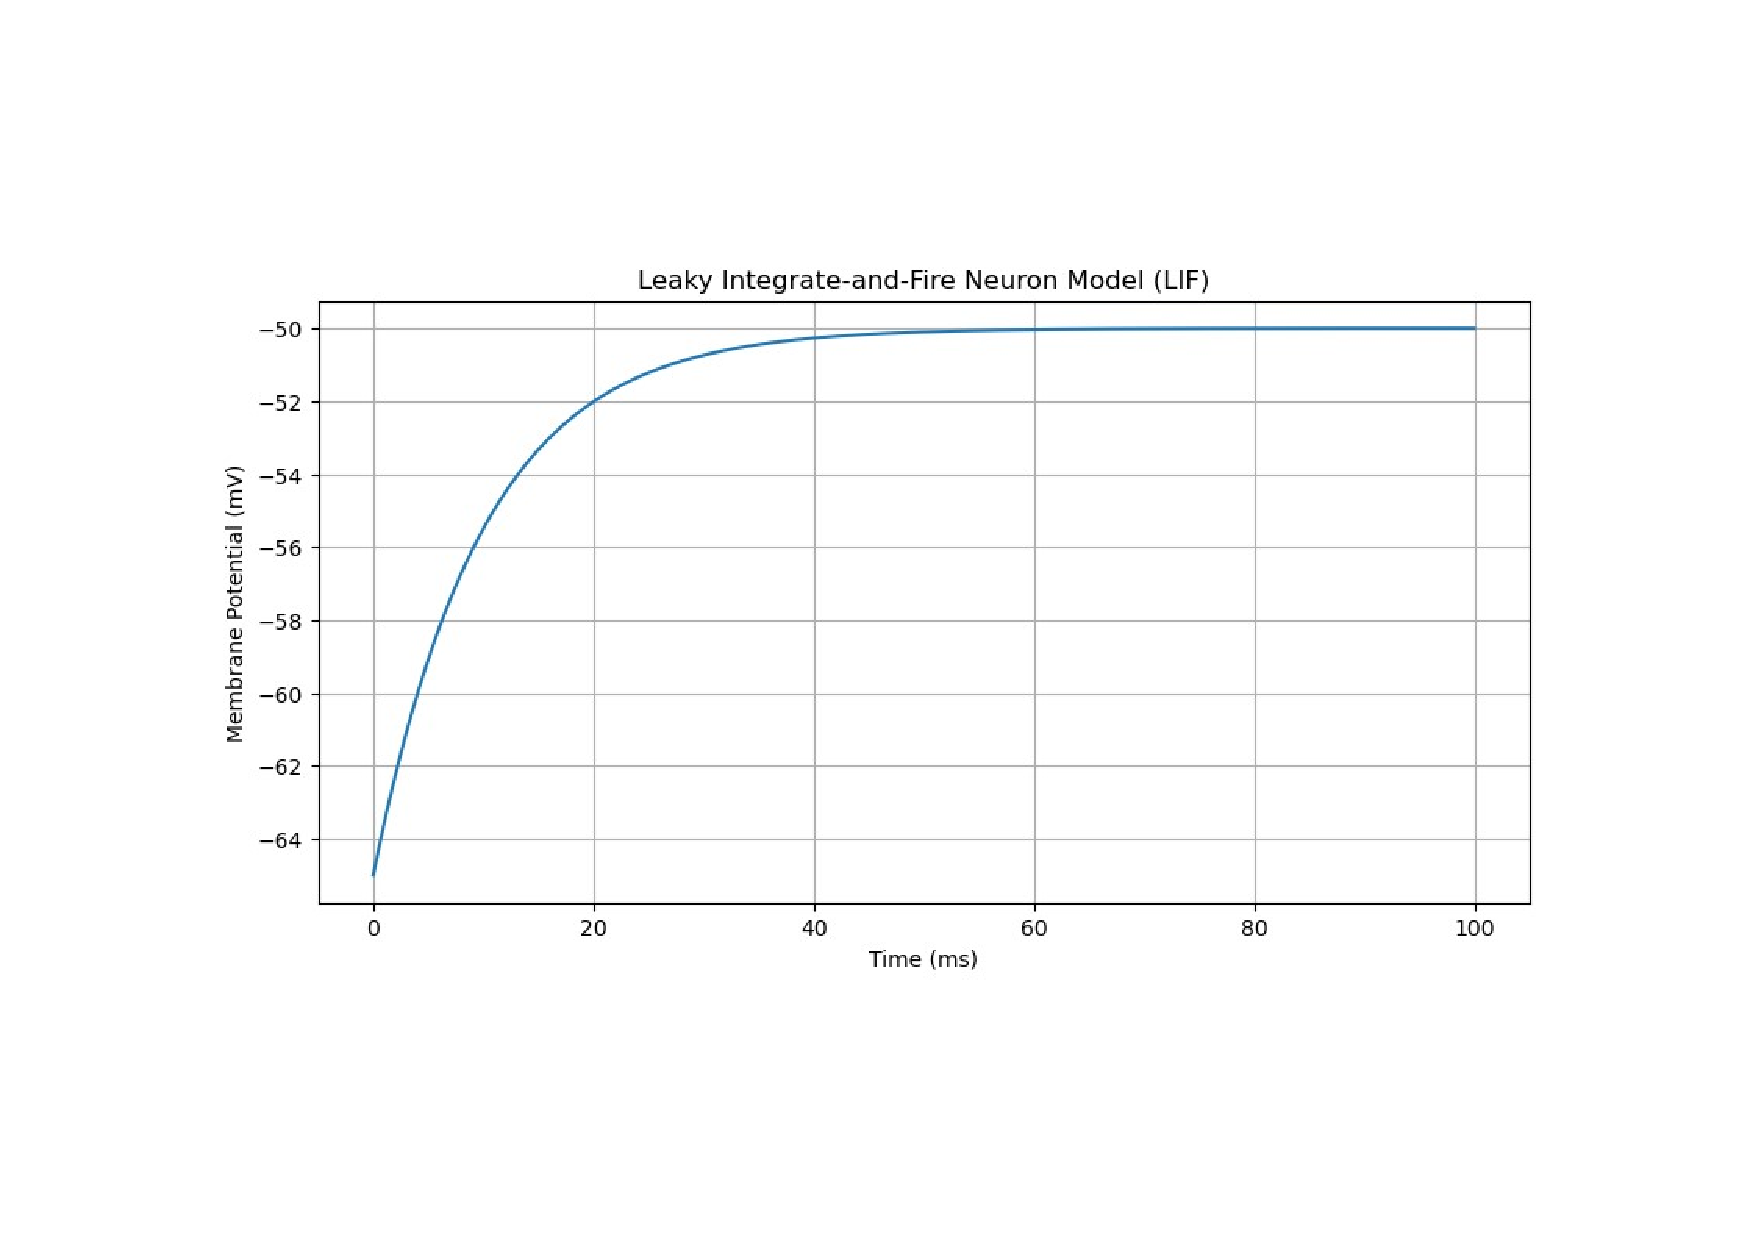
\includegraphics[width=2.5in]{image1.pdf} 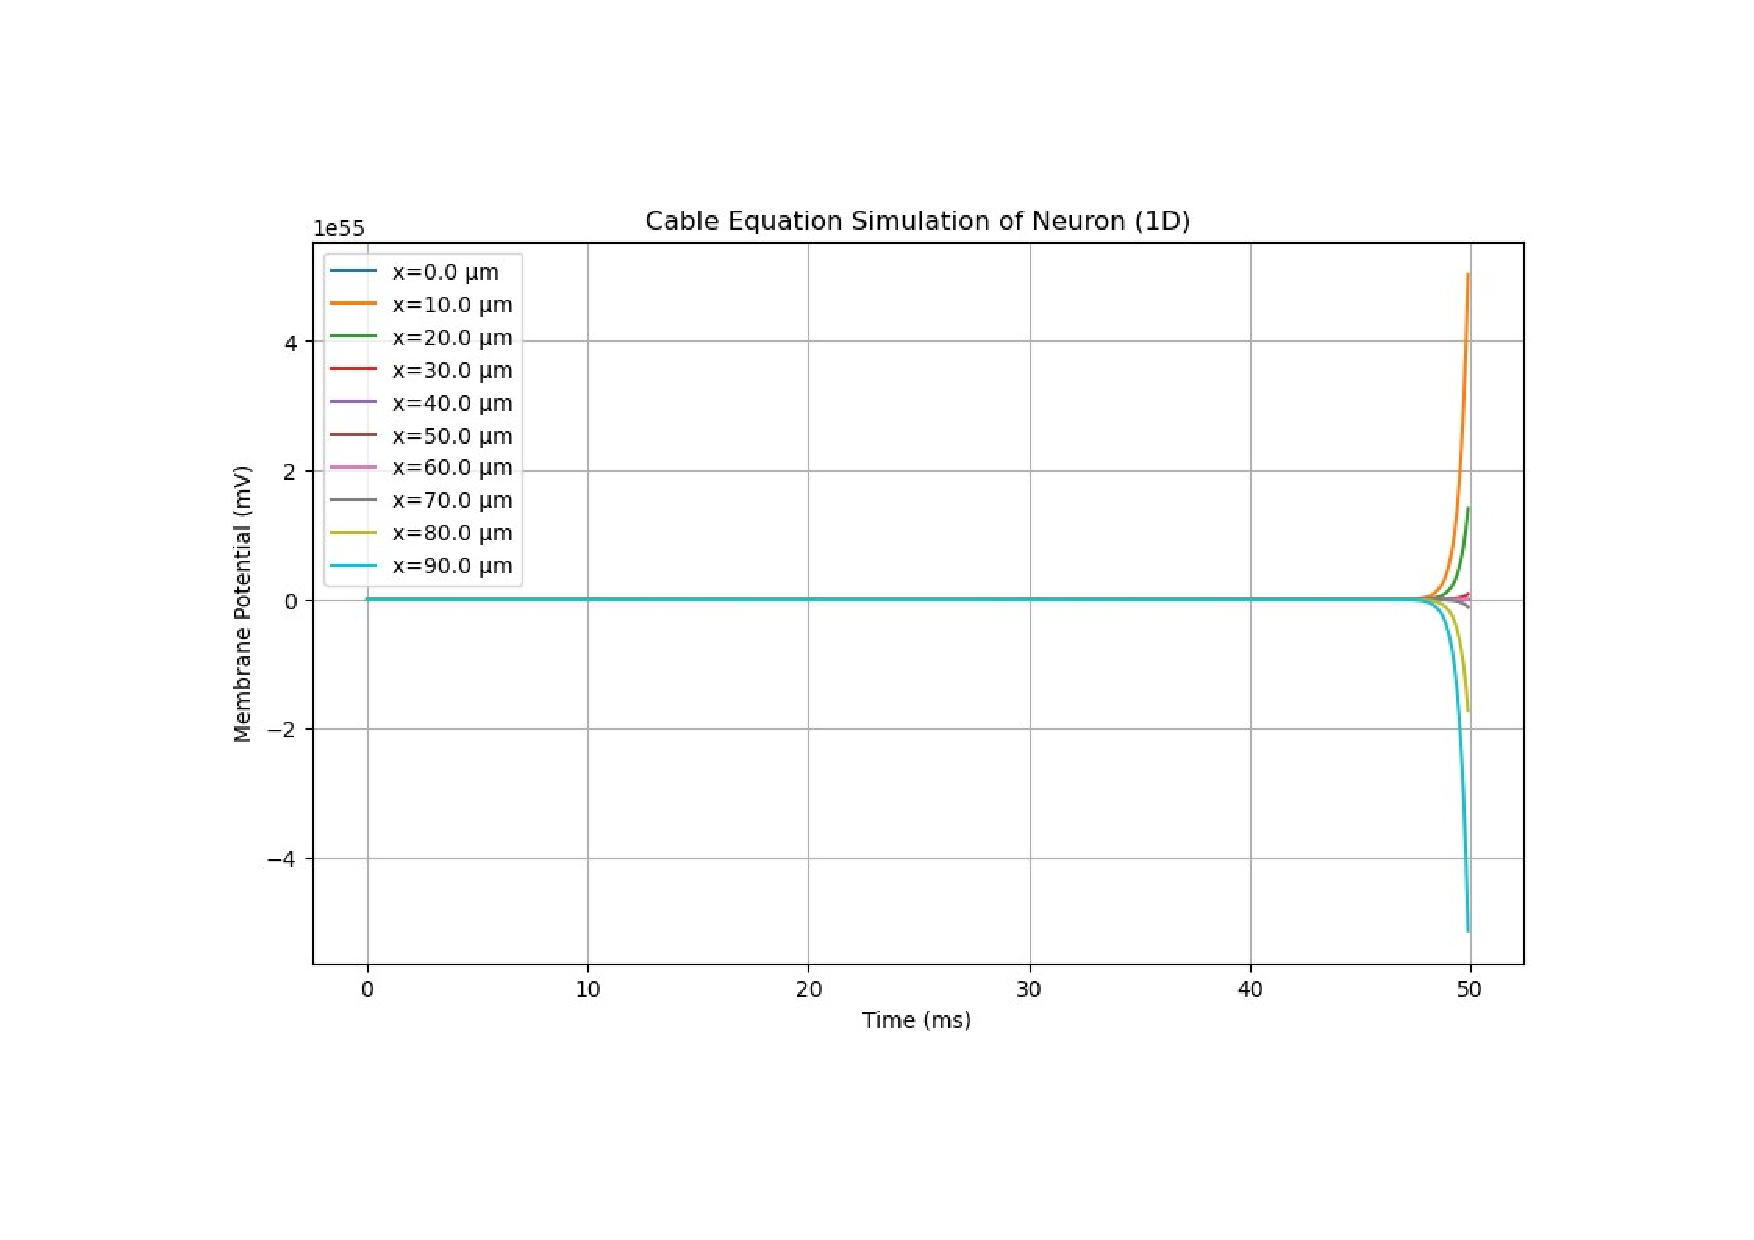
\includegraphics[width=2.5in] {image2.pdf} 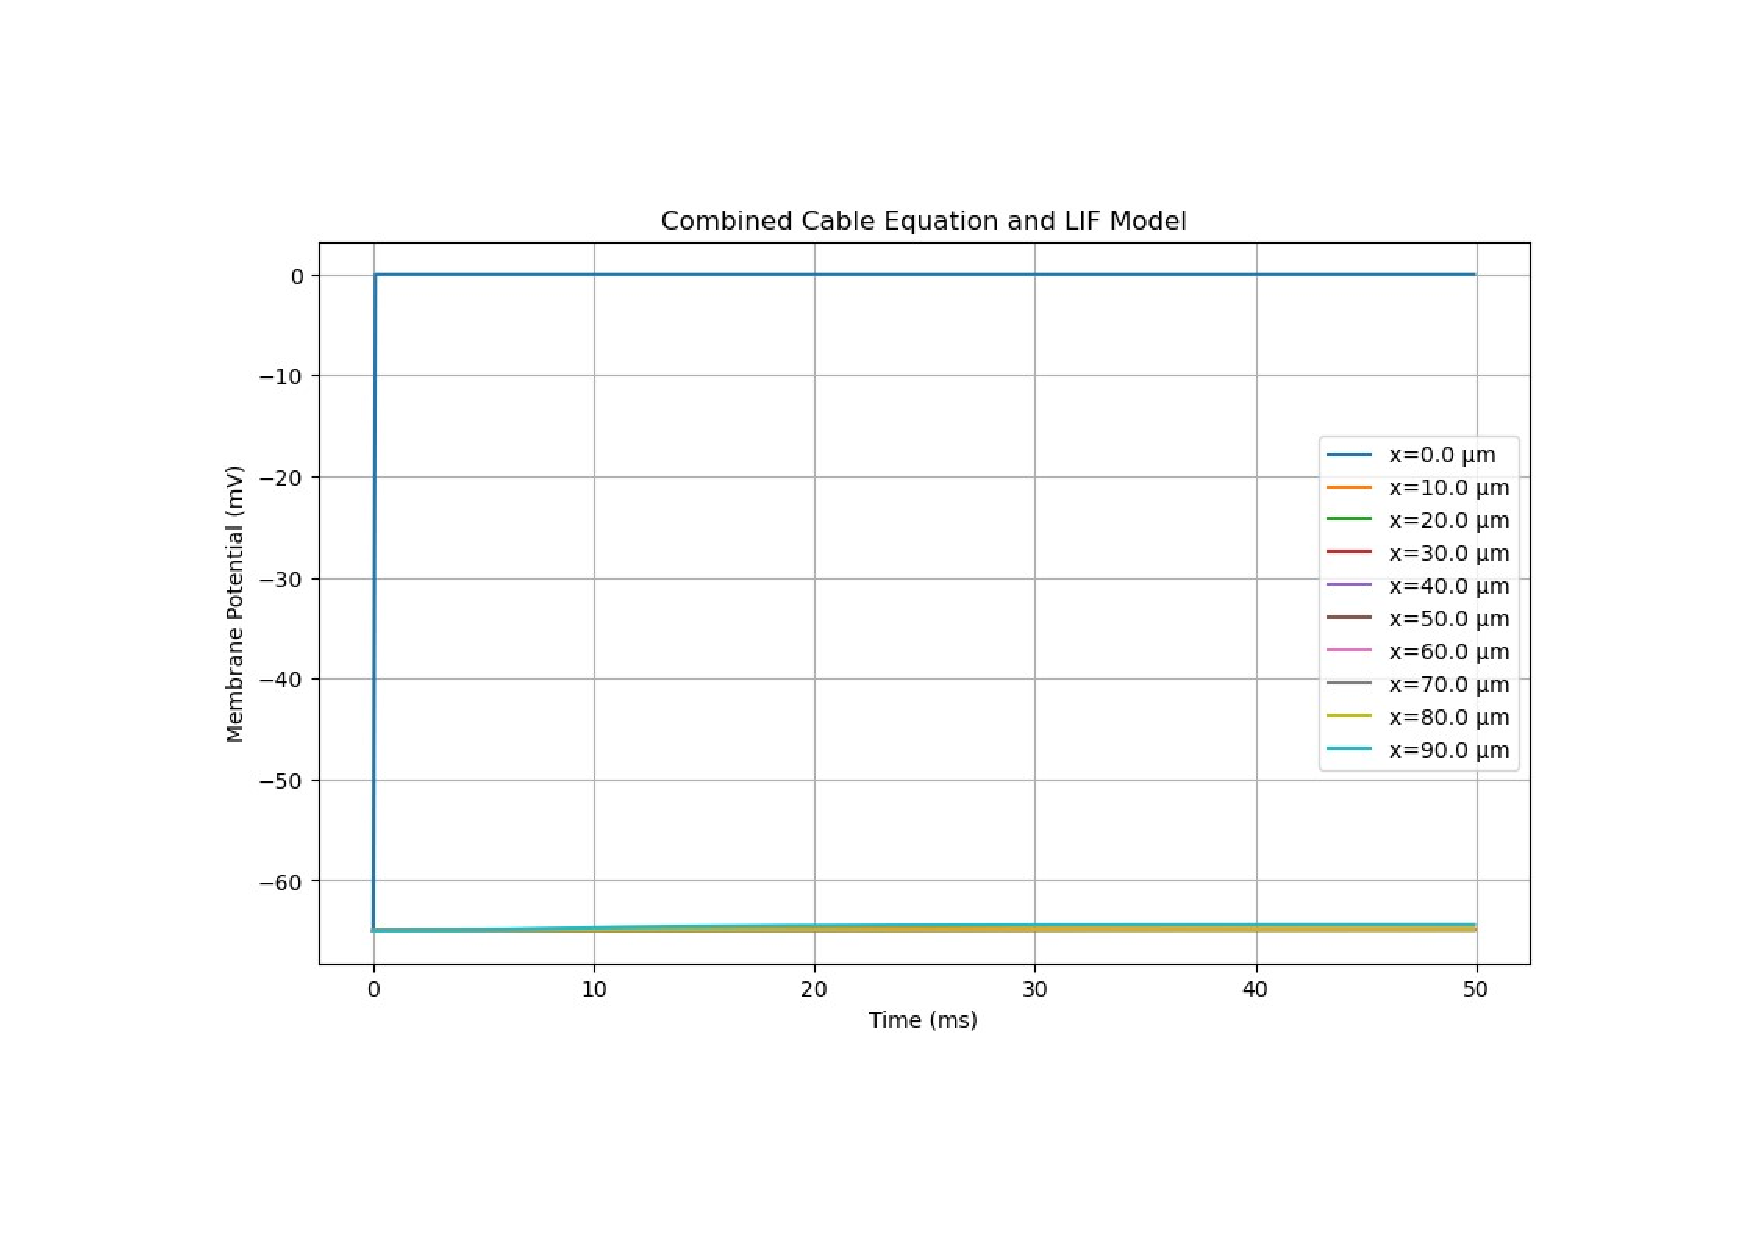
\includegraphics[width=2.5in]{image3.pdf}
\caption{{\bf (A)} 漏电积分放电(LIF)模型中膜电位的时间动态,其中神经元整合外部刺激并产生动作电位。}
\caption{{\bf (B)} 由电缆方程建模的动作电位沿神经元轴突的空间传播,展示了电信号如何随距离减弱。}
\caption{{\bf (C)} 神经元的组合时空动态,其中LIF模型和电缆方程被整合以模拟更真实的神经元活动。}
\end{figure}
\subsection*{4.1 LIF模型结果}

\begin{itemize}
    \item \textbf{图解说明}:这个图展示了LIF(Leaky Integrate-and-Fire)模型中神经元的膜电位随时间的变化。
    \begin{itemize}
        \item 横坐标是时间(ms),纵坐标是膜电位(mV)。
        \item 初始时,膜电位从静息电位(约 -65mV)开始随着时间逐渐增加。
        \item 当外部刺激以恒定电流形式施加时,膜电位逐渐上升,最终接近稳定状态。
    \end{itemize}
    \item \textbf{图中观察到的现象}:
    \begin{enumerate}
        \item \textbf{时间常数}:曲线呈现出典型的指数增加趋势,表明膜电位变化主要受到电容和膜电阻的影响。上升过程中的弯曲形态由膜时间常数 $\tau_m$ 决定。
        \item \textbf{稳定状态}:由于输入电流是恒定的,膜电位会接近一个稳定值,但不会达到阈值(-50mV)。说明在这个模拟中,外部电流不足以触发神经元的动作电位。
    \end{enumerate}
    \item \textbf{生物学意义}:该图反映了一个典型神经元在持续输入下的膜电位变化过程。LIF模型描述了神经元如何整合输入电流并在没有达到阈值时停止放电的情况。
\end{itemize}

\subsection*{4.2 电缆方程结果}

\begin{itemize}
    \item \textbf{图解说明}:这个图展示了电缆方程模拟的动作电位在神经元不同位置随时间的变化情况。
    \begin{itemize}
        \item 横坐标是时间(ms),纵坐标是膜电位(mV)。
        \item 不同颜色的曲线代表神经元不同位置(从 0 到 90$\mu$m)的膜电位变化。
    \end{itemize}
    \item \textbf{图中观察到的现象}:
    \begin{enumerate}
        \item \textbf{时间和空间上的电位变化}:在靠近电流注入点(例如 $x=10\mu m$)的地方,电位变化较大,而距离较远的位置(例如 $x=90\mu m$)电位变化趋于减弱。
        \item \textbf{信号的衰减}:随着距离的增加,电信号逐渐衰减。由于电缆方程中包含了电阻和电容的影响,远离电流注入点的位置无法保持同样的电位上升幅度。
    \end{enumerate}
    \item \textbf{生物学意义}:这个结果反映了电信号在神经元内的传播方式。由于电缆方程考虑了电阻和电容的影响,信号在沿轴突或树突传播的过程中会逐渐衰减。这种现象在真实生物神经元中尤为常见,是影响神经信号传输效率的重要因素。
\end{itemize}

\subsection*{4.3 组合LIF和电缆方程结果}

\begin{itemize}
    \item \textbf{图解说明}:这个图结合了电缆方程和LIF模型,展示了在神经元的不同位置上膜电位随时间的变化。
    \begin{itemize}
        \item 横坐标是时间(ms),纵坐标是膜电位(mV)。
        \item 不同曲线代表了不同位置上的膜电位变化。
    \end{itemize}
    \item \textbf{图中观察到的现象}:
    \begin{enumerate}
        \item \textbf{信号在不同位置的动态}:不同位置的膜电位变化幅度不同,但在初始时间点处有显著的电位增加。这是因为结合了LIF模型,当膜电位超过某个阈值时,触发了动作电位的产生。
        \item \textbf{动作电位的触发和复位}:在某些位置(例如靠近电流输入点的位置),膜电位达到阈值并触发动作电位后,电位迅速复位,体现了LIF模型中的“触发-复位”特性。
    \end{enumerate}
    \item \textbf{生物学意义}:结合LIF模型和电缆方程,能够更好地描述神经元对外部刺激的综合响应。图中的电位变化既体现了时间上的积累效应(LIF模型),又结合了空间上的传播和衰减特性(电缆方程)。这使得模型在描述神经信号如何通过复杂的神经元结构传播时更加逼真。
\end{itemize}


%%%-----------------------------------------------------------------
\section*{5. \textbf{讨论}}

\subsection*{5.1 组合模型的意义}

本研究将漏电积分放电(LIF)模型与电缆方程相结合,为理解神经元的时空动态提供了一个更为全面的框架。LIF模型能够有效地捕捉单个神经元随时间对输入刺激的电活动响应,而电缆方程则刻画了电信号沿树突或轴突的空间传播特性。通过将这两种模型相结合,我们可以模拟神经元如何在时间和空间维度上整合信号,这种结合更贴近神经元在真实生物系统中的行为表现。

结合模型的一个重要意义在于,它可以描述信号的集成与传播过程,而这种集成与传播在信息处理和传递中至关重要。例如,在神经系统中,神经元需要整合多个突触输入,生成的动作电位再通过轴突传递至下游神经元,进而实现复杂的神经计算和行为响应。本研究所建立的组合模型不仅考虑了时间动态,还将空间传播纳入了建模范围,使得对神经元行为的描述更加逼真且具有生物学合理性。

此外,这种组合模型还为多尺度的神经活动模拟提供了基础。在宏观层面,LIF模型可以用于描述神经网络中的放电模式;而在微观层面,电缆方程可以用于研究单个神经元内的电信号传播。因此,本研究的组合模型为理解神经元从分子尺度到系统尺度的多层次行为提供了新思路。

\subsection*{5.2 局限性}

尽管结合LIF模型与电缆方程为神经元行为的建模提供了更多的细节和准确性,但该模型仍然存在一些局限性。首先,LIF模型是一个相对简化的神经元模型,虽然它能够描述膜电位的累积和动作电位的触发,但忽略了许多重要的生物学细节,例如钠离子和钾离子通道的动态过程以及神经元的复杂树突结构。这些特性在更复杂的神经元模型中(如Hodgkin-Huxley模型)能够得到更为详细的描述。

其次,在电缆方程中,我们采用了一维空间近似,假设神经元为一条沿轴向传播的均匀电缆,而实际的神经元形态可能十分复杂,具有多分支的树突和不同的几何形状。此外,我们使用了显式有限差分方法来求解电缆方程,这种方法在某些条件下可能不够稳定,时间和空间步长的选择对结果的精度有较大影响,存在数值误差的可能性。

最后,本研究的组合模型并未考虑突触输入的空间分布和时间动态特性,而这些因素在真实神经元的信号处理过程中至关重要。突触输入的空间异质性和时间动态特性可以显著影响神经元的响应模式。因此,将这些生物学特性纳入未来的模型中将是进一步提高模型生物学合理性的重要方向。

%%%-----------------------------------------------------------------
\section*{6. \textbf{结论}}

本研究通过结合漏电积分放电(LIF)模型和电缆方程,建立了一个能够同时描述神经元时间动态和空间传播特性的组合模型。LIF模型有效地描述了神经元对外部刺激的整合与放电行为,而电缆方程则模拟了电信号在树突和轴突中的空间传播过程。数值模拟结果显示,该组合模型能够捕捉神经元在时间和空间上的复杂动态特性,揭示了电信号在神经元中的集成和传播过程,具有良好的生物学合理性。

结合模型的结果表明,神经元的电活动不仅受到时间维度上的输入变化影响,还受到空间维度上传导特性的制约。这一研究结果为理解神经系统中信号的时空整合机制提供了新的视角。此外,组合模型的成功实现也为进一步研究复杂神经元网络的时空行为提供了理论基础和计算框架。

未来的研究可以考虑引入更多生物学细节,例如离子通道动力学和突触输入的异质性,以进一步提高模型的生物学逼真度。同时,可以将本研究的模型应用于多神经元网络中,探索在网络层次上的复杂行为,例如同步化、振荡模式等。这将有助于进一步理解神经系统中的信息处理和传递机制,从而推进脑科学领域的研究。

%%%-----------------------------------------------------------------
\section*{附录A: 实验代码}

以下是用于实现漏电积分放电(LIF)模型和电缆方程的Python代码.

% 在文档中插入代码
\lstinputlisting[language=Python]{code.py}

该代码模拟了神经元在不同位置上的膜电位随时间的变化,结合了LIF模型的时间整合特性与电缆方程的空间传播特性,以实现对神经元时空动态的全面模拟。

\end{document}